%% ══════════════════════════════════════════════════════════════
%%  CHAPTER 15 — SYSTEM VISUALIZATIONS
%% ══════════════════════════════════════════════════════════════
\chapter{System Visualizations}
\label{ch:visualization}

\section{Full System Diagram}
\label{sec:viz:system}

\begin{figure}[H]
\centering
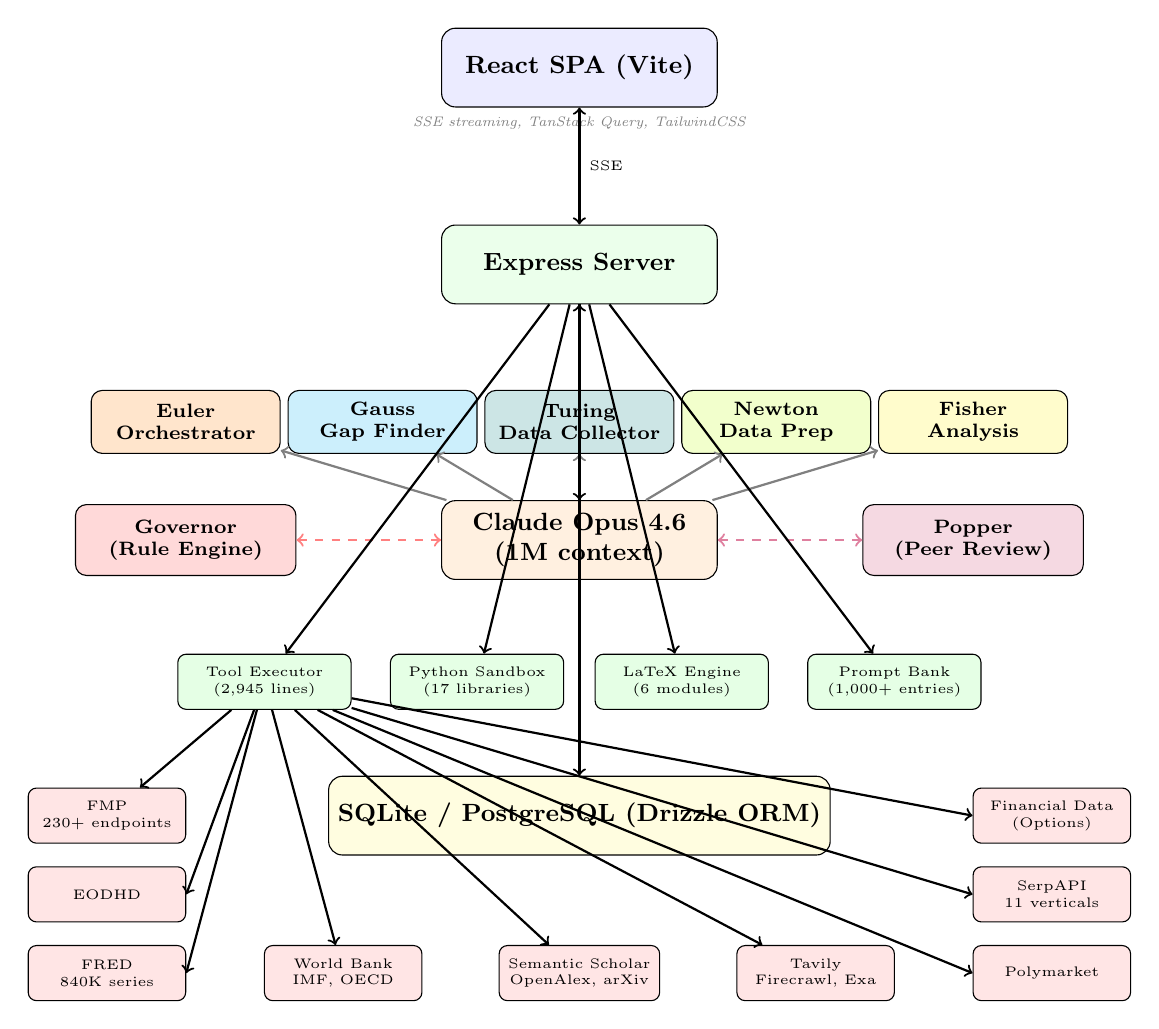
\begin{tikzpicture}[
  box/.style={draw, rounded corners=4pt, minimum width=2.8cm, minimum height=0.9cm, align=center, font=\scriptsize},
  bigbox/.style={draw, rounded corners=5pt, minimum width=3.5cm, minimum height=1cm, align=center, font=\small\bfseries},
  agent/.style={draw, rounded corners=4pt, minimum width=2.4cm, minimum height=0.8cm, align=center, font=\scriptsize\bfseries, fill=blue!15},
  service/.style={draw, rounded corners=3pt, minimum width=2.2cm, minimum height=0.7cm, align=center, font=\tiny, fill=green!10},
  ext/.style={draw, rounded corners=3pt, minimum width=2cm, minimum height=0.7cm, align=center, font=\tiny, fill=red!10},
  arrow/.style={->, thick},
  darrow/.style={<->, thick},
  note/.style={font=\tiny\itshape, text=gray},
]

% ── Client Layer ──
\node[bigbox, fill=blue!8] (client) at (0,11) {React SPA (Vite)};
\node[note] at (0,10.3) {SSE streaming, TanStack Query, TailwindCSS};

% ── Server Layer ──
\node[bigbox, fill=green!8] (server) at (0,8.5) {Express Server};

% ── Agents ──
\node[agent, fill=orange!20] (euler) at (-5,6.5) {Euler\\Orchestrator};
\node[agent, fill=cyan!20] (gauss) at (-2.5,6.5) {Gauss\\Gap Finder};
\node[agent, fill=teal!20] (turing) at (0,6.5) {Turing\\Data Collector};
\node[agent, fill=lime!20] (newton) at (2.5,6.5) {Newton\\Data Prep};
\node[agent, fill=yellow!20] (fisher) at (5,6.5) {Fisher\\Analysis};

% ── Governor & Popper ──
\node[box, fill=red!15, font=\scriptsize\bfseries] (governor) at (-5,5) {Governor\\(Rule Engine)};
\node[box, fill=purple!15, font=\scriptsize\bfseries] (popper) at (5,5) {Popper\\(Peer Review)};

% ── Claude API ──
\node[bigbox, fill=orange!12] (claude) at (0,5) {Claude Opus 4.6\\(1M context)};

% ── Service Layer ──
\node[service] (toolexec) at (-4,3.2) {Tool Executor\\(2,945 lines)};
\node[service] (python) at (-1.3,3.2) {Python Sandbox\\(17 libraries)};
\node[service] (latex) at (1.3,3.2) {LaTeX Engine\\(6 modules)};
\node[service] (promptbank) at (4,3.2) {Prompt Bank\\(1,000+ entries)};

% ── Storage ──
\node[bigbox, fill=yellow!12] (db) at (0,1.5) {SQLite / PostgreSQL (Drizzle ORM)};

% ── External APIs ──
\node[ext] (fmp) at (-6,1.5) {FMP\\230+ endpoints};
\node[ext] (eodhd) at (-6,0.5) {EODHD};
\node[ext] (fred) at (-6,-0.5) {FRED\\840K series};
\node[ext] (wb) at (-3,-0.5) {World Bank\\IMF, OECD};
\node[ext] (acad) at (0,-0.5) {Semantic Scholar\\OpenAlex, arXiv};
\node[ext] (web) at (3,-0.5) {Tavily\\Firecrawl, Exa};
\node[ext] (poly) at (6,-0.5) {Polymarket};
\node[ext] (serpapi) at (6,0.5) {SerpAPI\\11 verticals};
\node[ext] (findata) at (6,1.5) {Financial Data\\(Options)};

% ── Arrows ──
\draw[darrow] (client) -- node[right, font=\tiny] {SSE} (server);
\draw[darrow] (server) -- (claude);
\draw[arrow, gray] (claude) -- (euler);
\draw[arrow, gray] (claude) -- (gauss);
\draw[arrow, gray] (claude) -- (turing);
\draw[arrow, gray] (claude) -- (newton);
\draw[arrow, gray] (claude) -- (fisher);
\draw[darrow, dashed, red!50] (governor) -- (claude);
\draw[darrow, dashed, purple!50] (popper) -- (claude);
\draw[arrow] (server) -- (toolexec);
\draw[arrow] (server) -- (python);
\draw[arrow] (server) -- (latex);
\draw[arrow] (server) -- (promptbank);
\draw[arrow] (server) -- (db);
\draw[arrow] (toolexec) -- (fmp);
\draw[arrow] (toolexec) -- (eodhd.east);
\draw[arrow] (toolexec) -- (fred.east);
\draw[arrow] (toolexec) -- (wb);
\draw[arrow] (toolexec) -- (acad);
\draw[arrow] (toolexec) -- (web);
\draw[arrow] (toolexec) -- (poly.west);
\draw[arrow] (toolexec) -- (serpapi.west);
\draw[arrow] (toolexec) -- (findata.west);

\end{tikzpicture}
\caption{Complete \autoscholar system architecture diagram showing all agents, services, storage, and external integrations.}
\label{fig:full-system}
\end{figure}

\section{Pipeline Flow Diagram}
\label{sec:viz:pipeline}

\begin{figure}[H]
\centering
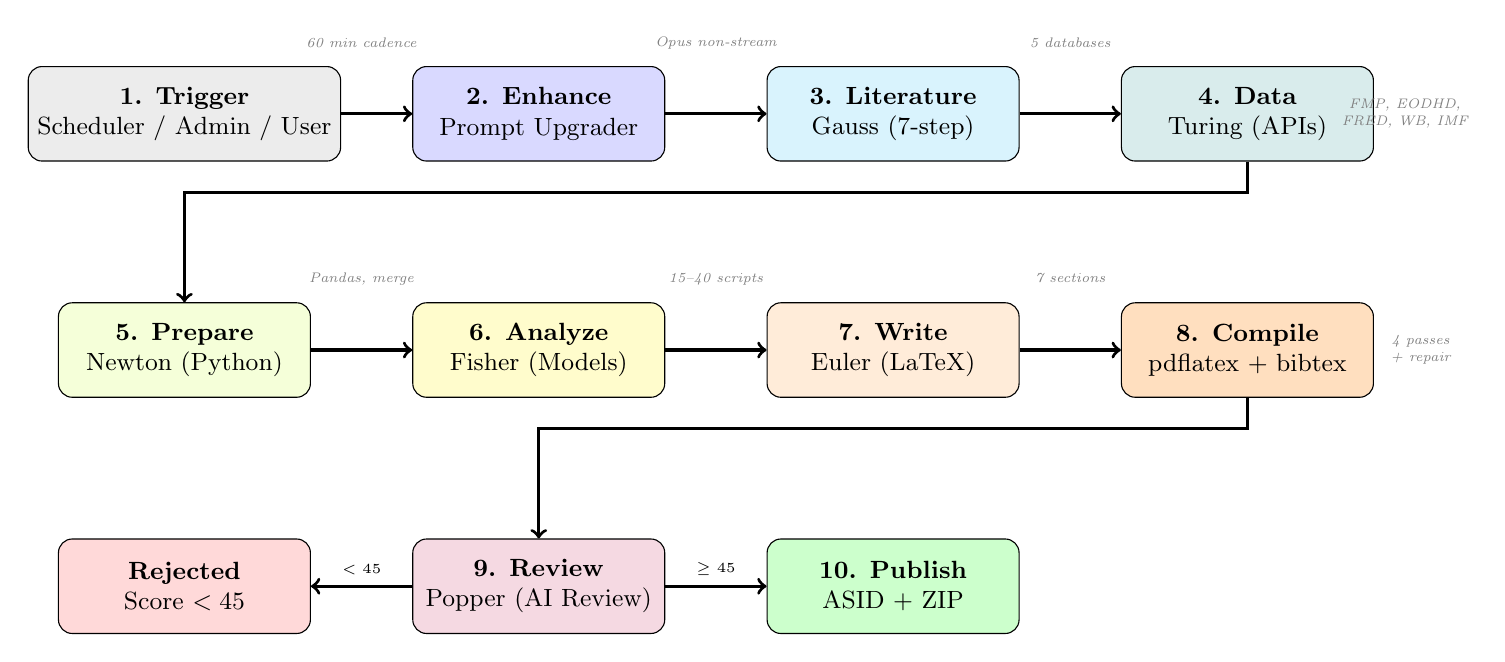
\begin{tikzpicture}[
  phase/.style={draw, rounded corners=5pt, minimum width=3.2cm, minimum height=1.2cm, align=center, font=\small},
  arrow/.style={->, very thick},
  label/.style={font=\tiny\itshape, text=gray},
]

% Phase boxes
\node[phase, fill=gray!15] (trigger) at (0,0) {\textbf{1. Trigger}\\Scheduler / Admin / User};
\node[phase, fill=blue!15] (enhance) at (4.5,0) {\textbf{2. Enhance}\\Prompt Upgrader};
\node[phase, fill=cyan!15] (gauss) at (9,0) {\textbf{3. Literature}\\Gauss (7-step)};
\node[phase, fill=teal!15] (turing) at (13.5,0) {\textbf{4. Data}\\Turing (APIs)};

\node[phase, fill=lime!15] (newton) at (0,-3) {\textbf{5. Prepare}\\Newton (Python)};
\node[phase, fill=yellow!20] (fisher) at (4.5,-3) {\textbf{6. Analyze}\\Fisher (Models)};
\node[phase, fill=orange!15] (write) at (9,-3) {\textbf{7. Write}\\Euler (LaTeX)};
\node[phase, fill=orange!25] (compile) at (13.5,-3) {\textbf{8. Compile}\\pdflatex + bibtex};

\node[phase, fill=purple!15] (review) at (4.5,-6) {\textbf{9. Review}\\Popper (AI Review)};
\node[phase, fill=green!20] (publish) at (9,-6) {\textbf{10. Publish}\\ASID + ZIP};
\node[phase, fill=red!15] (reject) at (0,-6) {\textbf{Rejected}\\Score $< 45$};

% Arrows
\draw[arrow] (trigger) -- (enhance);
\draw[arrow] (enhance) -- (gauss);
\draw[arrow] (gauss) -- (turing);
\draw[arrow] (turing) -- ++(0,-1) -| (newton);
\draw[arrow] (newton) -- (fisher);
\draw[arrow] (fisher) -- (write);
\draw[arrow] (write) -- (compile);
\draw[arrow] (compile) -- ++(0,-1) -| (review);
\draw[arrow] (review) -- node[above, font=\tiny] {$\geq 45$} (publish);
\draw[arrow] (review) -- node[above, font=\tiny] {$< 45$} (reject);

% Labels
\node[label] at (2.25,0.9) {60 min cadence};
\node[label] at (6.75,0.9) {Opus non-stream};
\node[label] at (11.25,0.9) {5 databases};
\node[label, align=center] at (15.5,0) {FMP, EODHD,\\FRED, WB, IMF};
\node[label] at (2.25,-2.1) {Pandas, merge};
\node[label] at (6.75,-2.1) {15--40 scripts};
\node[label] at (11.25,-2.1) {7 sections};
\node[label, align=center] at (15.7,-3) {4 passes\\+ repair};

\end{tikzpicture}
\caption{End-to-end paper generation pipeline with all 10 phases.}
\label{fig:pipeline-flow}
\end{figure}

\section{Agent Interaction Diagram}
\label{sec:viz:agents}

\begin{figure}[H]
\centering
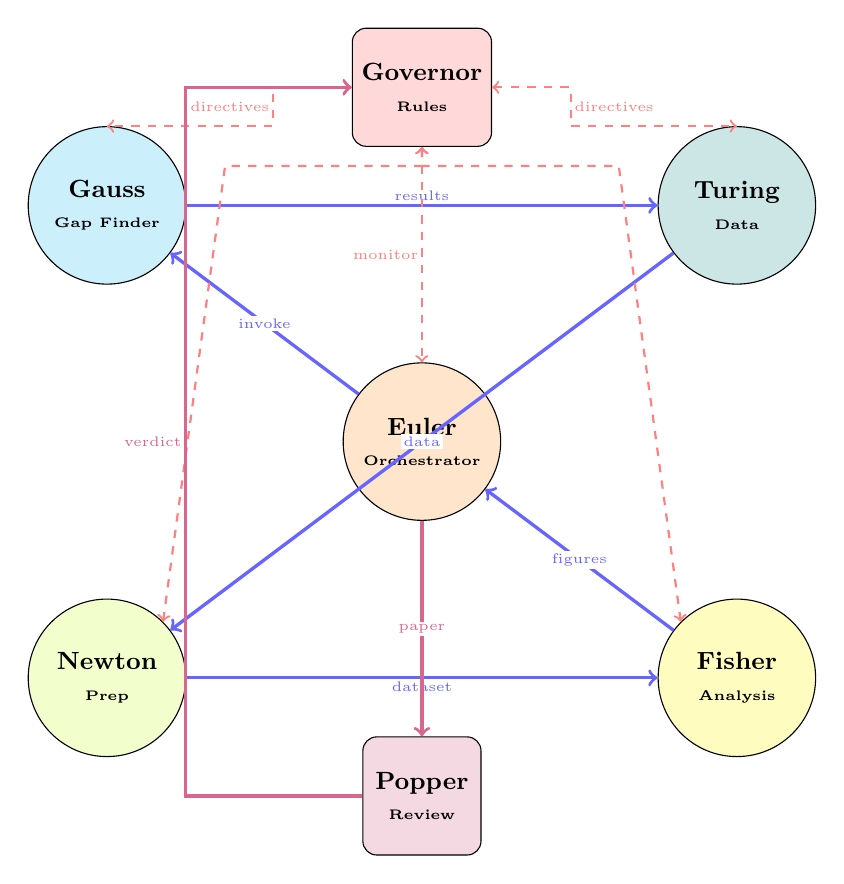
\begin{tikzpicture}[
  agent/.style={draw, circle, minimum size=2cm, align=center, font=\small\bfseries},
  arrow/.style={->, thick},
  darrow/.style={<->, thick, dashed},
  label/.style={font=\tiny, midway, fill=white, inner sep=1pt},
]

% Agents
\node[agent, fill=orange!20] (euler) at (0,0) {Euler\\{\tiny Orchestrator}};
\node[agent, fill=cyan!20] (gauss) at (-4,3) {Gauss\\{\tiny Gap Finder}};
\node[agent, fill=teal!20] (turing) at (4,3) {Turing\\{\tiny Data}};
\node[agent, fill=lime!20] (newton) at (-4,-3) {Newton\\{\tiny Prep}};
\node[agent, fill=yellow!25] (fisher) at (4,-3) {Fisher\\{\tiny Analysis}};
\node[agent, fill=red!15, rectangle, rounded corners=5pt, minimum size=1.5cm] (governor) at (0,4.5) {Governor\\{\tiny Rules}};
\node[agent, fill=purple!15, rectangle, rounded corners=5pt, minimum size=1.5cm] (popper) at (0,-4.5) {Popper\\{\tiny Review}};

% Sequential handoff
\draw[arrow, blue!60, very thick] (euler) -- node[label] {invoke} (gauss);
\draw[arrow, blue!60, very thick] (gauss) -- node[label, above] {results} (turing);
\draw[arrow, blue!60, very thick] (turing) -- node[label] {data} (newton);
\draw[arrow, blue!60, very thick] (newton) -- node[label, below] {dataset} (fisher);
\draw[arrow, blue!60, very thick] (fisher) -- node[label] {figures} (euler);

% Governor oversight
\draw[darrow, red!50] (governor) -- node[label, left] {monitor} (euler);
\draw[darrow, red!50] (governor.west) -- +(-1,0) |- node[label, left, pos=0.25] {directives} (gauss.north);
\draw[darrow, red!50] (governor.east) -- +(1,0) |- node[label, right, pos=0.25] {directives} (turing.north);
\draw[darrow, red!50] (governor) -- +(0,-1) -- +(-2.5,-1) -- (newton.north east);
\draw[darrow, red!50] (governor) -- +(0,-1) -- +(2.5,-1) -- (fisher.north west);

% Popper review
\draw[arrow, purple!60, very thick] (euler) -- node[label] {paper} (popper);
\draw[arrow, purple!60, very thick] (popper) -- +(-3,0) |- node[label, left, pos=0.25] {verdict} (governor);

\end{tikzpicture}
\caption{Agent interaction patterns showing sequential handoff (blue), governor oversight (red dashed), and Popper review feedback (purple).}
\label{fig:agent-interaction}
\end{figure}

\section{Data Flow Diagram}
\label{sec:viz:dataflow}

\begin{figure}[H]
\centering
\begin{tikzpicture}[
  store/.style={draw, cylinder, shape border rotate=90, minimum width=1.8cm, minimum height=1.2cm, align=center, font=\tiny, aspect=0.3},
  process/.style={draw, rounded corners=3pt, minimum width=2.2cm, minimum height=0.7cm, align=center, font=\tiny},
  ext/.style={draw, rounded corners=3pt, minimum width=1.8cm, minimum height=0.6cm, align=center, font=\tiny, fill=red!8},
  arrow/.style={->, thick},
]

% External sources
\node[ext] (apis) at (-6,4) {Financial APIs\\FMP, EODHD, FRED};
\node[ext] (macro) at (-6,2.5) {Macro APIs\\WB, IMF, OECD};
\node[ext] (acad) at (-6,1) {Academic DBs\\S2, OA, arXiv, CR};
\node[ext] (web) at (-6,-0.5) {Web Sources\\Tavily, Firecrawl, Exa};

% Processes
\node[process, fill=teal!15] (collect) at (-2,2.5) {Turing\\Data Collection};
\node[process, fill=lime!15] (prep) at (2,2.5) {Newton\\Data Prep};
\node[process, fill=yellow!20] (analyze) at (2,0.5) {Fisher\\Analysis};
\node[process, fill=orange!15] (write) at (2,-1.5) {Euler\\Writing};
\node[process, fill=orange!25] (compile) at (6,-1.5) {LaTeX\\Compiler};

% Storage
\node[store, fill=yellow!12] (db) at (6,4) {SQLite/PG\\Database};
\node[store, fill=blue!8] (files) at (6,2) {File System\\downloads/};
\node[store, fill=green!8] (zip) at (6,0) {Project ZIP\\RRE Archive};

% Arrows
\draw[arrow] (apis) -- (collect);
\draw[arrow] (macro) -- (collect);
\draw[arrow] (acad) -- (collect);
\draw[arrow] (web) -- (collect);
\draw[arrow] (collect) -- node[above, font=\tiny] {raw data} (prep);
\draw[arrow] (collect) -- (files);
\draw[arrow] (prep) -- node[right, font=\tiny] {datasets} (analyze);
\draw[arrow] (prep) -- (files);
\draw[arrow] (analyze) -- node[right, font=\tiny] {results, figs} (write);
\draw[arrow] (analyze) -- (files);
\draw[arrow] (write) -- node[above, font=\tiny] {LaTeX} (compile);
\draw[arrow] (compile) -- (zip);
\draw[arrow] (compile) -- (db);
\draw[arrow] (write) -- ++(0,-1) -| (db);

\end{tikzpicture}
\caption{Data flow from external sources through processing stages to persistent storage.}
\label{fig:data-flow}
\end{figure}

\section{Governor Decision Flow}
\label{sec:viz:governor}

\begin{figure}[H]
\centering
\begin{tikzpicture}[
  decision/.style={draw, diamond, minimum width=2.5cm, minimum height=1.5cm, align=center, font=\tiny, inner sep=1pt},
  action/.style={draw, rounded corners=3pt, minimum width=2cm, minimum height=0.6cm, align=center, font=\tiny},
  arrow/.style={->, thick},
]

\node[action, fill=blue!15] (input) at (0,6) {Tool Result\\Received};
\node[decision, fill=yellow!15] (stage) at (0,4) {Detect\\Stage?};
\node[decision, fill=red!15] (pyerr) at (-4,2) {Python\\Error?};
\node[decision, fill=red!15] (dataerr) at (0,2) {Data\\Issue?};
\node[decision, fill=red!15] (latexerr) at (4,2) {LaTeX\\Error?};
\node[decision, fill=orange!15] (budget) at (-4,0) {Retry\\Budget?};
\node[action, fill=green!15] (cont) at (0,0) {Continue};
\node[action, fill=red!20] (force) at (-4,-1.5) {Force\\Finalize};
\node[action, fill=orange!15] (switch) at (-1,-1.5) {Switch\\Profile};
\node[action, fill=purple!15] (inject) at (2,-1.5) {Inject\\Directive};
\node[action, fill=red!25] (block) at (5,-1.5) {Block\\Publication};

\draw[arrow] (input) -- (stage);
\draw[arrow] (stage) -- (pyerr);
\draw[arrow] (stage) -- (dataerr);
\draw[arrow] (stage) -- (latexerr);
\draw[arrow] (pyerr) -- node[left, font=\tiny] {yes} (budget);
\draw[arrow] (pyerr) -- node[above, font=\tiny] {no} (cont);
\draw[arrow] (dataerr) -- node[right, font=\tiny] {no} (cont);
\draw[arrow] (dataerr) -- node[left, font=\tiny] {yes} (switch);
\draw[arrow] (latexerr) -- node[left, font=\tiny] {yes} (inject);
\draw[arrow] (latexerr) |- node[right, font=\tiny, pos=0.3] {fatal} (block);
\draw[arrow] (budget) -- node[left, font=\tiny] {empty} (force);
\draw[arrow] (budget) -- node[above, font=\tiny] {ok} (switch);

\end{tikzpicture}
\caption{Governor decision flow showing error detection, budget checking, and action selection.}
\label{fig:governor-flow}
\end{figure}

\section{Storage Schema Diagram}
\label{sec:viz:schema}

\begin{figure}[H]
\centering
\begin{tikzpicture}[
  table/.style={draw, rectangle split, rectangle split parts=2, minimum width=3cm, align=center, font=\tiny, rounded corners=2pt},
  arrow/.style={->, thick, gray},
]

% Core tables
\node[table, fill=blue!10] (users) at (-5,6) {
  \textbf{users}
  \nodepart{second}
  id, username, email\\passwordHash, role\\apiKey, token
};

\node[table, fill=green!10] (sessions) at (0,6) {
  \textbf{conversationSessions}
  \nodepart{second}
  id, userId, sessionId\\title, messageCount\\totalTokens, totalCost
};

\node[table, fill=green!10] (messages) at (5,6) {
  \textbf{messages}
  \nodepart{second}
  id, sessionId, role\\content, sources
};

\node[table, fill=orange!10] (papers) at (-5,2.5) {
  \textbf{publishedPapers}
  \nodepart{second}
  id, title, abstract\\domain, template\\latexSections, bibtex\\asid, projectZipPath
};

\node[table, fill=purple!10] (reviews) at (0,2.5) {
  \textbf{peerReviews}
  \nodepart{second}
  id, paperId\\overallScore\\recommendation\\detailedScores
};

\node[table, fill=red!10] (runs) at (5,2.5) {
  \textbf{paperRuns}
  \nodepart{second}
  id, status, prompt\\sessionId, heartbeat\\popperScore\\governorState
};

\node[table, fill=yellow!10] (apikeys) at (-5,-1) {
  \textbf{apiKeys}
  \nodepart{second}
  id, keyHash, label\\scopes, rateLimit\\usageCount
};

\node[table, fill=gray!10] (config) at (0,-1) {
  \textbf{siteConfig}
  \nodepart{second}
  key, value
};

\node[table, fill=cyan!10] (shared) at (5,-1) {
  \textbf{sharedReports}
  \nodepart{second}
  id, shareId\\question, answer\\sources, toolResults
};

% Relationships
\draw[arrow] (users) -- node[above, font=\tiny] {1:N} (sessions);
\draw[arrow] (sessions) -- node[above, font=\tiny] {1:N} (messages);
\draw[arrow] (papers) -- node[above, font=\tiny] {1:1} (reviews);
\draw[arrow] (papers.east) -- ++(1,0) |- node[font=\tiny, pos=0.25, right] {via sessionId} (runs.west);

\end{tikzpicture}
\caption{Core database schema relationships (simplified, 20+ tables total).}
\label{fig:schema}
\end{figure}

\section{Tool Ecosystem Map}
\label{sec:viz:tools}

\begin{figure}[H]
\centering
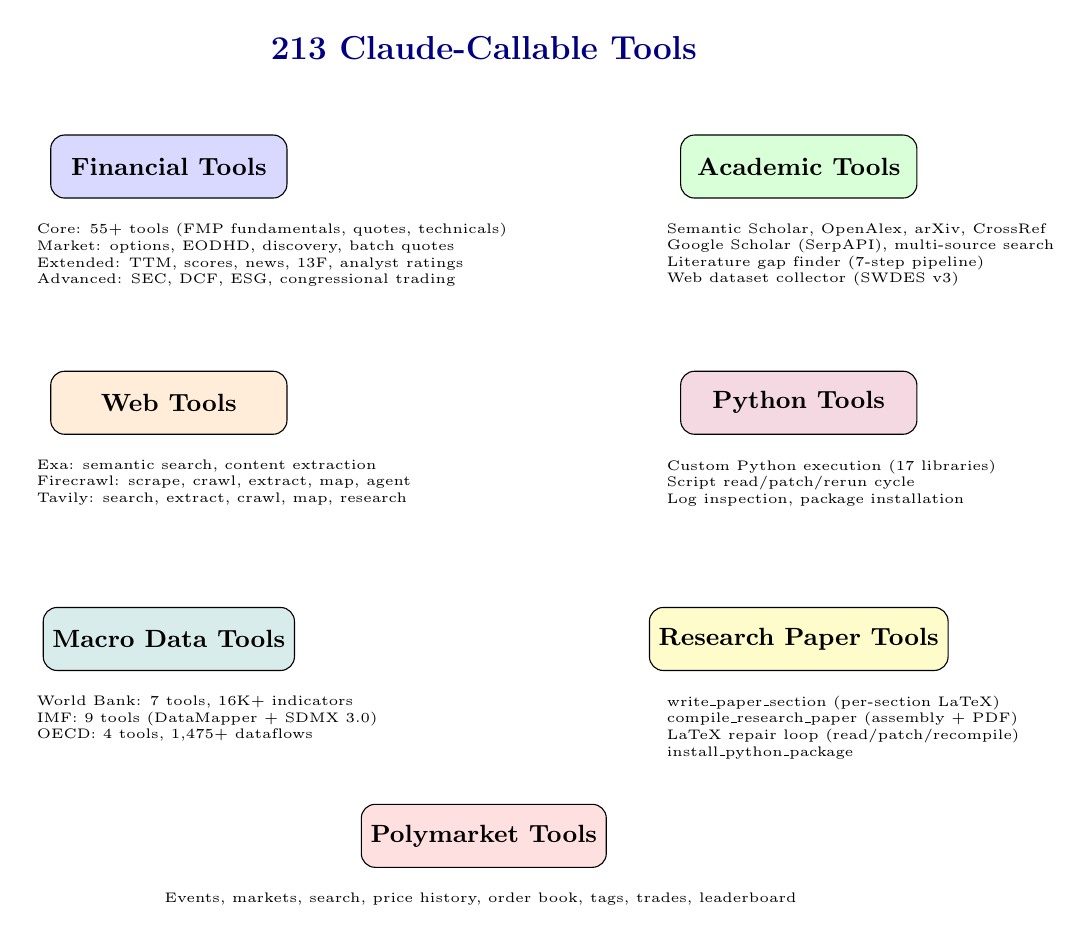
\begin{tikzpicture}[
  cat/.style={draw, rounded corners=5pt, minimum width=3cm, minimum height=0.8cm, align=center, font=\small\bfseries},
  item/.style={font=\tiny, align=left},
]

\node[cat, fill=blue!15] (fin) at (-4,5) {Financial Tools};
\node[item, anchor=north west] at (-5.8,4.4) {
  Core: 55+ tools (FMP fundamentals, quotes, technicals)\\
  Market: options, EODHD, discovery, batch quotes\\
  Extended: TTM, scores, news, 13F, analyst ratings\\
  Advanced: SEC, DCF, ESG, congressional trading
};

\node[cat, fill=green!15] (acad) at (4,5) {Academic Tools};
\node[item, anchor=north west] at (2.2,4.4) {
  Semantic Scholar, OpenAlex, arXiv, CrossRef\\
  Google Scholar (SerpAPI), multi-source search\\
  Literature gap finder (7-step pipeline)\\
  Web dataset collector (SWDES v3)
};

\node[cat, fill=orange!15] (web) at (-4,2) {Web Tools};
\node[item, anchor=north west] at (-5.8,1.4) {
  Exa: semantic search, content extraction\\
  Firecrawl: scrape, crawl, extract, map, agent\\
  Tavily: search, extract, crawl, map, research
};

\node[cat, fill=purple!15] (py) at (4,2) {Python Tools};
\node[item, anchor=north west] at (2.2,1.4) {
  Custom Python execution (17 libraries)\\
  Script read/patch/rerun cycle\\
  Log inspection, package installation
};

\node[cat, fill=teal!15] (macro) at (-4,-1) {Macro Data Tools};
\node[item, anchor=north west] at (-5.8,-1.6) {
  World Bank: 7 tools, 16K+ indicators\\
  IMF: 9 tools (DataMapper + SDMX 3.0)\\
  OECD: 4 tools, 1,475+ dataflows
};

\node[cat, fill=yellow!20] (paper) at (4,-1) {Research Paper Tools};
\node[item, anchor=north west] at (2.2,-1.6) {
  write\_paper\_section (per-section LaTeX)\\
  compile\_research\_paper (assembly + PDF)\\
  LaTeX repair loop (read/patch/recompile)\\
  install\_python\_package
};

\node[cat, fill=red!12] (poly) at (0,-3.5) {Polymarket Tools};
\node[item, anchor=north] at (0,-4.1) {
  Events, markets, search, price history, order book, tags, trades, leaderboard
};

% Total
\node[font=\large\bfseries, text=NavyBlue] at (0,6.5) {213 Claude-Callable Tools};

\end{tikzpicture}
\caption{Tool ecosystem organized by category showing the breadth of \autoscholar's capabilities.}
\label{fig:tool-map}
\end{figure}
